\documentclass{standalone}
\usepackage{tikz}
\usetikzlibrary{patterns, positioning}


\begin{document}
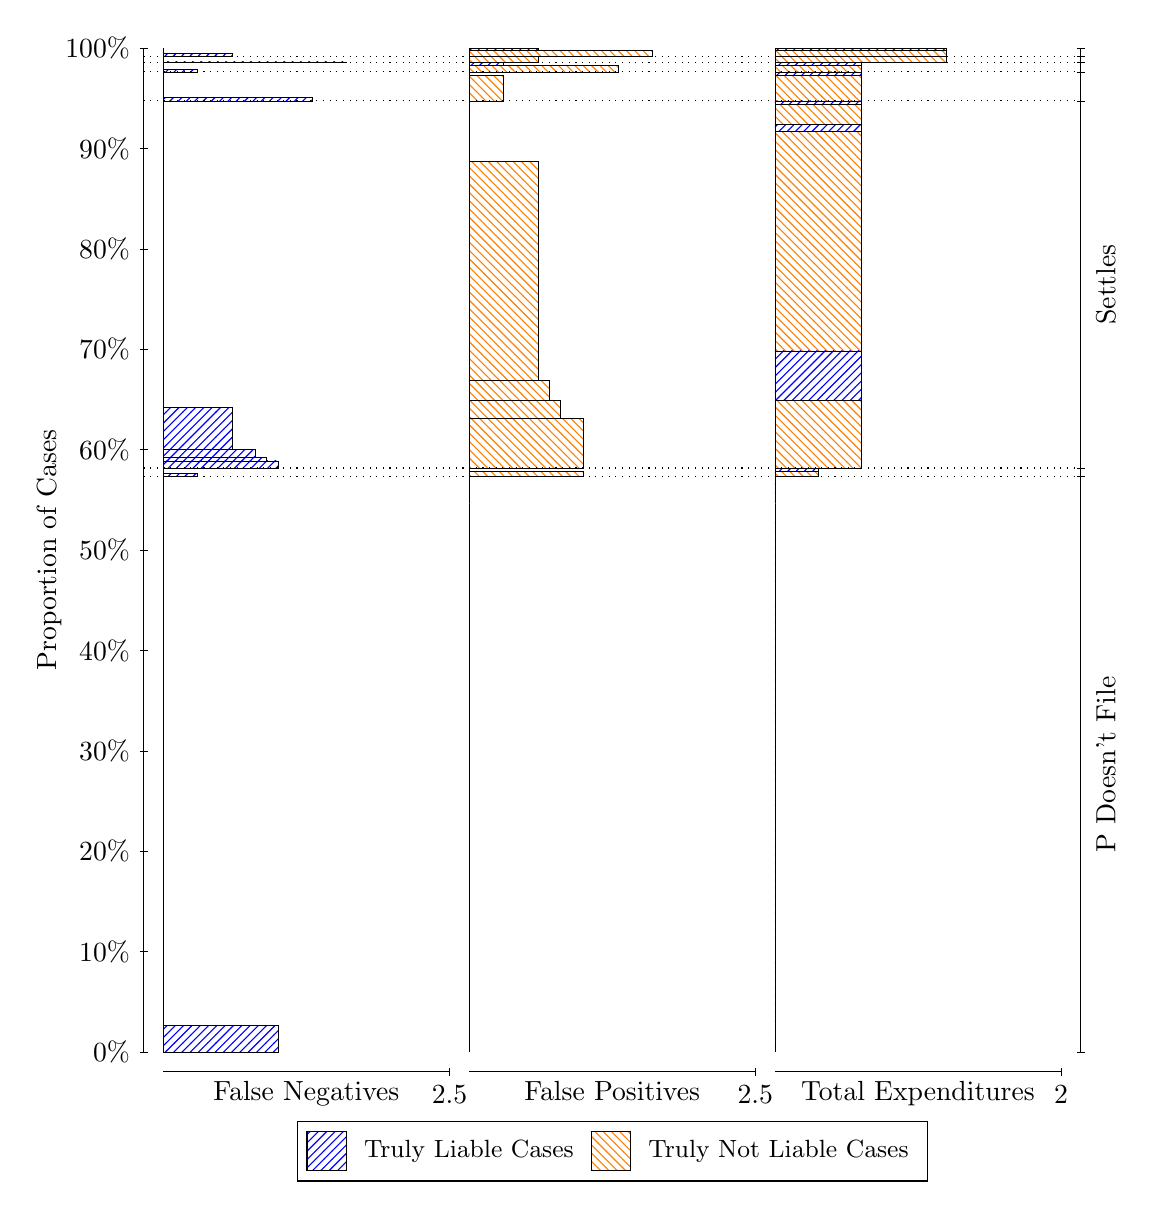
\begin{tikzpicture}
\draw[black, very thin] (1.5,1.75) -- (1.5,14.5);
\node[rotate=90, text=black, anchor=center] at (0.3, 8.125) {Proportion of Cases};
\draw[black, very thin] (1.45,1.75) -- (1.55,1.75);
\node[text=black, anchor=east] at (1.45, 1.75) {0\%};
\draw[black, very thin] (1.45,3.025) -- (1.55,3.025);
\node[text=black, anchor=east] at (1.45, 3.025) {10\%};
\draw[black, very thin] (1.45,4.3) -- (1.55,4.3);
\node[text=black, anchor=east] at (1.45, 4.3) {20\%};
\draw[black, very thin] (1.45,5.575) -- (1.55,5.575);
\node[text=black, anchor=east] at (1.45, 5.575) {30\%};
\draw[black, very thin] (1.45,6.85) -- (1.55,6.85);
\node[text=black, anchor=east] at (1.45, 6.85) {40\%};
\draw[black, very thin] (1.45,8.125) -- (1.55,8.125);
\node[text=black, anchor=east] at (1.45, 8.125) {50\%};
\draw[black, very thin] (1.45,9.4) -- (1.55,9.4);
\node[text=black, anchor=east] at (1.45, 9.4) {60\%};
\draw[black, very thin] (1.45,10.675) -- (1.55,10.675);
\node[text=black, anchor=east] at (1.45, 10.675) {70\%};
\draw[black, very thin] (1.45,11.95) -- (1.55,11.95);
\node[text=black, anchor=east] at (1.45, 11.95) {80\%};
\draw[black, very thin] (1.45,13.225) -- (1.55,13.225);
\node[text=black, anchor=east] at (1.45, 13.225) {90\%};
\draw[black, very thin] (1.45,14.5) -- (1.55,14.5);
\node[text=black, anchor=east] at (1.45, 14.5) {100\%};

\draw[black, very thin] (13.4,1.75) -- (13.4,14.5);
\draw[black, very thin] (13.35,1.75) -- (13.45,1.75);
\node[anchor=west] at (13.35, 1.75) {};
\draw[black, very thin] (13.35,9.0567) -- (13.45,9.0567);
\node[anchor=west] at (13.35, 9.0567) {};
\draw[black, very thin] (13.35,9.1658) -- (13.45,9.1658);
\node[anchor=west] at (13.35, 9.1658) {};
\draw[black, very thin] (13.35,13.83) -- (13.45,13.83);
\node[anchor=west] at (13.35, 13.83) {};
\draw[black, very thin] (13.35,14.197) -- (13.45,14.197);
\node[anchor=west] at (13.35, 14.197) {};
\draw[black, very thin] (13.35,14.316) -- (13.45,14.316);
\node[anchor=west] at (13.35, 14.316) {};
\draw[black, very thin] (13.35,14.397) -- (13.45,14.397);
\node[anchor=west] at (13.35, 14.397) {};
\draw[black, very thin] (13.35,14.5) -- (13.45,14.5);
\node[anchor=west] at (13.35, 14.5) {};

\draw[black, very thin, pattern color=blue, pattern=north east lines] (1.75,1.75) rectangle (3.2033,2.0914);
\draw[black, very thin, pattern color=orange, pattern=north west lines] (1.75,2.0914) rectangle (1.75,9.0567);
\draw[black, very thin, pattern color=blue, pattern=north east lines] (1.75,9.0567) rectangle (2.186,9.1007);
\draw[black, very thin, pattern color=orange, pattern=north west lines] (1.75,9.1007) rectangle (1.75,9.1658);
\draw[black, very thin, pattern color=blue, pattern=north east lines] (1.75,9.1658) rectangle (3.2033,9.2571);
\draw[black, very thin, pattern color=blue, pattern=north east lines] (1.75,9.2571) rectangle (3.058,9.3023);
\draw[black, very thin, pattern color=blue, pattern=north east lines] (1.75,9.3023) rectangle (2.9127,9.4048);
\draw[black, very thin, pattern color=blue, pattern=north east lines] (1.75,9.4048) rectangle (2.622,9.9346);
\draw[black, very thin, pattern color=orange, pattern=north west lines] (1.75,9.9346) rectangle (1.75,13.83);
\draw[black, very thin, pattern color=blue, pattern=north east lines] (1.75,13.83) rectangle (3.6393,13.876);
\draw[black, very thin, pattern color=orange, pattern=north west lines] (1.75,13.876) rectangle (1.75,14.197);
\draw[black, very thin, pattern color=blue, pattern=north east lines] (1.75,14.197) rectangle (2.186,14.233);
\draw[black, very thin, pattern color=orange, pattern=north west lines] (1.75,14.233) rectangle (1.75,14.316);
\draw[black, very thin, pattern color=blue, pattern=north east lines] (1.75,14.316) rectangle (4.0753,14.324);
\draw[black, very thin, pattern color=orange, pattern=north west lines] (1.75,14.324) rectangle (1.75,14.397);
\draw[black, very thin, pattern color=blue, pattern=north east lines] (1.75,14.397) rectangle (2.622,14.428);
\draw[black, very thin, pattern color=orange, pattern=north west lines] (1.75,14.428) rectangle (1.75,14.5);
\draw[black, very thin, pattern color=orange, pattern=north west lines] (5.6333,1.75) rectangle (5.6333,8.7153);
\draw[black, very thin, pattern color=blue, pattern=north east lines] (5.6333,8.7153) rectangle (5.6333,9.0567);
\draw[black, very thin, pattern color=orange, pattern=north west lines] (5.6333,9.0567) rectangle (7.0867,9.1218);
\draw[black, very thin, pattern color=blue, pattern=north east lines] (5.6333,9.1218) rectangle (5.6333,9.1658);
\draw[black, very thin, pattern color=orange, pattern=north west lines] (5.6333,9.1658) rectangle (7.0867,9.7939);
\draw[black, very thin, pattern color=orange, pattern=north west lines] (5.6333,9.7939) rectangle (6.796,10.022);
\draw[black, very thin, pattern color=orange, pattern=north west lines] (5.6333,10.022) rectangle (6.6507,10.277);
\draw[black, very thin, pattern color=orange, pattern=north west lines] (5.6333,10.277) rectangle (6.5053,13.061);
\draw[black, very thin, pattern color=blue, pattern=north east lines] (5.6333,13.061) rectangle (5.6333,13.83);
\draw[black, very thin, pattern color=orange, pattern=north west lines] (5.6333,13.83) rectangle (6.0693,14.151);
\draw[black, very thin, pattern color=blue, pattern=north east lines] (5.6333,14.151) rectangle (5.6333,14.197);
\draw[black, very thin, pattern color=orange, pattern=north west lines] (5.6333,14.197) rectangle (7.5227,14.28);
\draw[black, very thin, pattern color=blue, pattern=north east lines] (5.6333,14.28) rectangle (6.0693,14.316);
\draw[black, very thin, pattern color=orange, pattern=north west lines] (5.6333,14.316) rectangle (6.5053,14.389);
\draw[black, very thin, pattern color=blue, pattern=north east lines] (5.6333,14.389) rectangle (5.6333,14.397);
\draw[black, very thin, pattern color=orange, pattern=north west lines] (5.6333,14.397) rectangle (7.9587,14.469);
\draw[black, very thin, pattern color=blue, pattern=north east lines] (5.6333,14.469) rectangle (6.5053,14.5);
\draw[black, very thin, pattern color=orange, pattern=north west lines] (9.5167,1.75) rectangle (9.5167,8.7153);
\draw[black, very thin, pattern color=blue, pattern=north east lines] (9.5167,8.7153) rectangle (9.5167,9.0567);
\draw[black, very thin, pattern color=orange, pattern=north west lines] (9.5167,9.0567) rectangle (10.062,9.1218);
\draw[black, very thin, pattern color=blue, pattern=north east lines] (9.5167,9.1218) rectangle (10.062,9.1658);
\draw[black, very thin, pattern color=orange, pattern=north west lines] (9.5167,9.1658) rectangle (10.607,10.022);
\draw[black, very thin, pattern color=blue, pattern=north east lines] (9.5167,10.022) rectangle (10.607,10.654);
\draw[black, very thin, pattern color=orange, pattern=north west lines] (9.5167,10.654) rectangle (10.607,13.438);
\draw[black, very thin, pattern color=blue, pattern=north east lines] (9.5167,13.438) rectangle (10.607,13.529);
\draw[black, very thin, pattern color=orange, pattern=north west lines] (9.5167,13.529) rectangle (10.607,13.785);
\draw[black, very thin, pattern color=blue, pattern=north east lines] (9.5167,13.785) rectangle (10.607,13.83);
\draw[black, very thin, pattern color=orange, pattern=north west lines] (9.5167,13.83) rectangle (10.607,14.151);
\draw[black, very thin, pattern color=blue, pattern=north east lines] (9.5167,14.151) rectangle (10.607,14.197);
\draw[black, very thin, pattern color=orange, pattern=north west lines] (9.5167,14.197) rectangle (10.607,14.28);
\draw[black, very thin, pattern color=blue, pattern=north east lines] (9.5167,14.28) rectangle (10.607,14.316);
\draw[black, very thin, pattern color=orange, pattern=north west lines] (9.5167,14.316) rectangle (11.697,14.389);
\draw[black, very thin, pattern color=blue, pattern=north east lines] (9.5167,14.389) rectangle (11.697,14.397);
\draw[black, very thin, pattern color=orange, pattern=north west lines] (9.5167,14.397) rectangle (11.697,14.469);
\draw[black, very thin, pattern color=blue, pattern=north east lines] (9.5167,14.469) rectangle (11.697,14.5);
\draw[black, dotted] (1.5,9.0567) -- (13.4,9.0567);
\draw[black, dotted] (1.5,9.1658) -- (13.4,9.1658);
\draw[black, dotted] (1.5,13.83) -- (13.4,13.83);
\draw[black, dotted] (1.5,14.197) -- (13.4,14.197);
\draw[black, dotted] (1.5,14.316) -- (13.4,14.316);
\draw[black, dotted] (1.5,14.397) -- (13.4,14.397);
\draw[black, very thin] (1.75,1.5) -- (5.3833,1.5);
\node[text=black, anchor=north] at (3.5667, 1.5) {False Negatives};
\draw[black, very thin] (5.3833,1.45) -- (5.3833,1.55);
\node[text=black, anchor=north] at (5.3833, 1.45) {2.5};

\draw[black, very thin] (5.6333,1.5) -- (9.2667,1.5);
\node[text=black, anchor=north] at (7.45, 1.5) {False Positives};
\draw[black, very thin] (9.2667,1.45) -- (9.2667,1.55);
\node[text=black, anchor=north] at (9.2667, 1.45) {2.5};

\draw[black, very thin] (9.5167,1.5) -- (13.15,1.5);
\node[text=black, anchor=north] at (11.333, 1.5) {Total Expenditures};
\draw[black, very thin] (13.15,1.45) -- (13.15,1.55);
\node[text=black, anchor=north] at (13.15, 1.45) {2};

\node[text=black, centered, rotate=90] at (13.72, 5.4034) {P Doesn't File};

\node[text=black, centered, rotate=90] at (13.72, 11.498) {Settles};





\draw (7.449999999999999,1.5) node[draw=none] (baseCoordinate) {};
\begin{scope}[align=center]
        \matrix[scale=0.5, draw=black, below=0.5cm of baseCoordinate, nodes={draw}, column sep=0.1cm]{
            \node[rectangle, draw, minimum width=0.5cm, minimum height=0.5cm, pattern color=blue, pattern=north east lines] {}; &
            \node[draw=none, font=\small, text=black] (B) {Truly Liable Cases}; &
            \node[rectangle, draw, minimum width=0.5cm, minimum height=0.5cm, pattern color=orange, pattern=north west lines] {}; &
            \node[draw=none, font=\small, text=black] (B) {Truly Not Liable Cases}; \\
            };
\end{scope}

\end{tikzpicture}
\end{document}